\documentclass[9pt,aspectratio=169,xcolor=table]{beamer}

%~~~~~~~~~~~~~~~~~~~~~~~~~~~~~~~~~~~~~~~~~~~~~~~~~~~~~~~~~~~~~~~~~~~~~~~~~~~~~~
% Use roboto Font (recommended)
\usepackage[sfdefault]{roboto}
\usepackage[utf8]{inputenc}
\usepackage[T1]{fontenc}
%~~~~~~~~~~~~~~~~~~~~~~~~~~~~~~~~~~~~~~~~~~~~~~~~~~~~~~~~~~~~~~~~~~~~~~~~~~~~~~

%~~~~~~~~~~~~~~~~~~~~~~~~~~~~~~~~~~~~~~~~~~~~~~~~~~~~~~~~~~~~~~~~~~~~~~~~~~~~~~
% Define where theme files are located. ('/styles')
\usepackage{styles/fluxmacros}
\usefolder{styles}
% Use Flux theme v0.1 beta
% Available style: asphalt, blue, red, green, gray
\usetheme[style=hunter]{flux}
%~~~~~~~~~~~~~~~~~~~~~~~~~~~~~~~~~~~~~~~~~~~~~~~~~~~~~~~~~~~~~~~~~~~~~~~~~~~~~~

%~~~~~~~~~~~~~~~~~~~~~~~~~~~~~~~~~~~~~~~~~~~~~~~~~~~~~~~~~~~~~~~~~~~~~~~~~~~~~~
% Extra packages
\usepackage{booktabs}
\usepackage{colortbl}
\usepackage{ragged2e}
\usepackage{amssymb}
\usepackage{multirow}
\usepackage{tikz}
\usetikzlibrary{arrows.meta, positioning, fit, backgrounds, calc, decorations.pathreplacing}
\setbeamertemplate{itemize items}[square]
\usepackage[scaled=.8]{beramono}
\usepackage{listings}
\usepackage{styles/lstlangarm}
\usepackage{array}
\usepackage{makecell}
\definecolor{bgcolor}{HTML}{F2E9E9}
% lstlangarm.sty references \color{mauve} for string literals but never defines
% it -- only fires when a listing contains a string. Define it here.
\definecolor{mauve}{rgb}{0.58,0,0.82}
% lstlangarm's C style sets commentstyle=green!20, which is unreadable on the
% pink listing background. Darken it globally.
\lstset{commentstyle=\color{green!45!black}}
% ragged-right fixed-width column -- must be defined in the preamble, never
% inside a frame (\newcolumntype's #1 breaks beamer's frame scanner)
\newcolumntype{R}[1]{>{\RaggedRight\arraybackslash}p{#1}}
%~~~~~~~~~~~~~~~~~~~~~~~~~~~~~~~~~~~~~~~~~~~~~~~~~~~~~~~~~~~~~~~~~~~~~~~~~~~~~~
% Table striping: odd rows white, even rows very light gray.
% Needs \documentclass[...,xcolor=table]{beamer} (beamer loads xcolor itself,
% so the option must go on the class, not \usepackage).
\definecolor{stripe}{gray}{0.94}
% \striped makes body rows alternate white, gray, white, ... starting white.
% \rowcolors counts from the first coloured body row; the header is not counted.
\newcommand{\striped}{\rowcolors{1}{white}{stripe}}
%~~~~~~~~~~~~~~~~~~~~~~~~~~~~~~~~~~~~~~~~~~~~~~~~~~~~~~~~~~~~~~~~~~~~~~~~~~~~~~

%~~~~~~~~~~~~~~~~~~~~~~~~~~~~~~~~~~~~~~~~~~~~~~~~~~~~~~~~~~~~~~~~~~~~~~~~~~~~~~
% TikZ block styles -- matches ch1/ch2
% Colour variables are named identically in the book's stm32primer.tex, so any
% tikzpicture using only the \tikzset{...} styles below can be copied verbatim
% between slides and book. Only the \definecolor/\colorlet VALUES differ: the
% book is printed, so it keeps every stroke pure black with muted fills. These
% slides are projected, so both fill AND stroke are bright and saturated to
% grab attention -- see stm32primer.tex for the print palette.
\definecolor{blkfill}{HTML}{DDEEDD}
\definecolor{blkline}{HTML}{355E3B}
\definecolor{accentfill}{HTML}{FFE0B2}
\definecolor{accentline}{HTML}{E65100}
\definecolor{memfill}{HTML}{DFF5DA}
\definecolor{memline}{HTML}{2E7D32}
\definecolor{cellfill}{HTML}{FFFFFF}
\definecolor{cellline}{HTML}{424242}
\definecolor{bitmaskfill}{HTML}{DCEBFF}
\definecolor{bitmaskline}{HTML}{1565C0}
\definecolor{bithitfill}{HTML}{FFE0B2}
\definecolor{bithitline}{HTML}{E65100}
\tikzset{
  blk/.style   = {rectangle, rounded corners=2pt, draw=blkline, fill=blkfill,
                  thick, align=center, font=\small, minimum height=9mm, inner sep=3pt},
  cpublk/.style= {rectangle, rounded corners=2pt, draw=accentline, fill=accentfill,
                  thick, align=center, font=\small\bfseries, minimum height=9mm, inner sep=3pt},
  memblk/.style= {rectangle, rounded corners=2pt, draw=memline, fill=memfill,
                  thick, align=center, font=\small, minimum height=9mm, inner sep=3pt},
  cell/.style  = {rectangle, draw=cellline, fill=cellfill, align=center,
                  font=\small\ttfamily, minimum height=7mm, inner sep=2pt},
  bitcell/.style={rectangle, draw=cellline, fill=cellfill, thick,
                  minimum width=5.4mm, minimum height=5.4mm, inner sep=0pt,
                  font=\scriptsize\ttfamily, anchor=center},
  bitmask/.style={bitcell, fill=bitmaskfill, draw=bitmaskline},
  bithit/.style ={bitcell, fill=bithitfill, draw=bithitline, font=\scriptsize\ttfamily\bfseries},
  rowlab/.style ={font=\scriptsize, text=Gray, anchor=east},
  oplab/.style  ={font=\scriptsize\itshape, text=Gray, anchor=west},
  lbl/.style   = {font=\scriptsize, text=Gray},
  flow/.style  = {-{Stealth[length=2mm]}, thick, draw=blkline},
  busline/.style={thick, draw=cellline},
}
% NOTE (theme quirks -- all fail SILENTLY, always page through the PDF):
%  - a second \\ inside a nested {...} group in a TikZ node breaks parsing
%  - {\small ...} wrapped around a nested itemize eats the frame title + list
%  - \usebeamercolor on a [plain] frame falls through to an unstyled default
%  - \newcolumntype inside a frame breaks beamer's frame scanner
%  - lstlisting needs \begin{frame}[fragile]
%  - a TikZ picture wider than its column silently overflows into neighbours
%~~~~~~~~~~~~~~~~~~~~~~~~~~~~~~~~~~~~~~~~~~~~~~~~~~~~~~~~~~~~~~~~~~~~~~~~~~~~~~

%%%%%%%%%%%%%%%%%%%%%%%%%%%%%%%%%%%
%% BEGIN CONDITIONAL COMPILATION %%
%%%%%%%%%%%%%%%%%%%%%%%%%%%%%%%%%%%
\newif\ifwebex
%\webextrue % uncomment to generate section separator
\ifwebex
\AtBeginSection[]{
  \begin{frame}
  \vfill
  \centering
  \begin{beamercolorbox}[sep=8pt,center,shadow=true,rounded=true]{title}
    \usebeamerfont{title}\insertsectionhead\par%
  \end{beamercolorbox}
  \vfill
  \end{frame}
}
\else
\AtBeginSection[]
{
{
    \setbeamercolor{background canvas}{bg=yellow!10}
    \begin{frame}[plain]
        \frametitle{Table of Contents}
        \tableofcontents[currentsection]
    \end{frame}
}
}
\fi
%%%%%%%%%%%%%%%%%%%%%%%%%%%%%%%%%%%
%% END CONDITIONAL COMPILATION   %%
%%%%%%%%%%%%%%%%%%%%%%%%%%%%%%%%%%%

%~~~~~~~~~~~~~~~~~~~~~~~~~~~~~~~~~~~~~~~~~~~~~~~~~~~~~~~~~~~~~~~~~~~~~~~~~~~~~~
% Information
\title{First Steps in Verilog}
\subtitle{\emph{Contemporary Digital Electronic Systems} --- Chapter 16}
\author{Mun\'{i}m Zabidi}
\institute{\color{primary}Faculty of Electrical Engineering, Universiti Teknologi Malaysia}
\date{\today}
\titlegraphic{assets/logoutmwhite.png}
\graphicspath{{.}{../fig/}}
%~~~~~~~~~~~~~~~~~~~~~~~~~~~~~~~~~~~~~~~~~~~~~~~~~~~~~~~~~~~~~~~~~~~~~~~~~~~~~~

\newcommand{\figh}[2]{\includegraphics[height=#1\textheight]{#2}}



\lstset{language=Verilog,basicstyle=\ttfamily\footnotesize,keywordstyle=\color{blue!60!black}\bfseries,commentstyle=\color{green!45!black}\itshape,backgroundcolor=\color{gray!8},frame=single,rulecolor=\color{gray!40},showstringspaces=false,columns=fullflexible,xleftmargin=0pt,framexleftmargin=2pt,aboveskip=0pt,belowskip=0pt}

\begin{document}

\titlepage

%===============================================================================
\section{Why This Chapter}
%===============================================================================

\begin{frame}{Why This Chapter Matters}
  \begin{columns}[c]
  \begin{column}{.47\textwidth}
    Every circuit in Chapters 4--15 could be drawn as a schematic. In practice designers write them in a \alert{hardware description language} (HDL) and let a synthesis tool produce the gate-level netlist. This chapter is a \emph{first exposure} to synthesizable Verilog: enough to describe, simulate and synthesise circuits you already know how to build.
  \end{column}
  \begin{column}{.51\textwidth}
    \begin{block}{After this chapter, you can:}
    {\small
    \begin{enumerate}\itemsep2pt
      \item Write a \texttt{module} with named inputs and outputs.
      \item Describe combinational logic three ways (\texttt{assign}, \texttt{always @(*)} with \texttt{case}, gate primitives) and say which fits which situation.
      \item Describe an edge-triggered register with \texttt{always @(posedge clk)}.
      \item Write and read a three-process FSM.
    \end{enumerate}}
    \end{block}
  \end{column}
  \end{columns}
  \vspace{1mm}
  {\footnotesize \textbf{Scope.} A conservative, synthesizable subset of Verilog-2005 that mainstream tools accept: continuous assignments, \texttt{always} blocks, \texttt{case} statements. It is not a complete HDL reference.}
\end{frame}

\begin{frame}{An Opening Question}
  \leavevmode\vspace{4mm}
  \begin{center}
  \fbox{\parbox{.78\textwidth}{\centering\vspace{2mm}
  \large If Verilog ``looks like C'', why does it compile to \alert{logic gates} instead of CPU instructions?
  \vspace{2mm}}}
  \end{center}
  \vspace{4mm}
  What is Verilog really describing?
\end{frame}

\begin{frame}{Hardware Is Concurrent}
  \begin{itemize}\small\itemsep4pt
    \item Verilog is \alert{not} a program whose statements run in order. Every \texttt{assign} and every \texttt{always} block exists \emph{simultaneously} in the hardware, like a schematic where every component is always powered.
    \item Inside one \texttt{always} block, textual order implies an order of effect (last assignment wins), but there is no program counter.
    \item You define ``what the hardware \emph{is}'', not ``what steps to execute''.
  \end{itemize}
  \begin{alertblock}{Syntactically valid $\ne$ synthesizable}
    \small A simulator accepts \texttt{initial} blocks, delays, floating-point literals, dynamic array sizes, non-constant loop bounds. No synthesis tool can build them. ``My simulation passes'' is not evidence the design fits a real FPGA: the \alert{synthesis report} is the ground truth.
  \end{alertblock}
\end{frame}

\begin{frame}{From Hardware Idea to Verilog}
  \centering\small\striped
  \begin{tabular}{@{}lR{.28\textwidth}R{.34\textwidth}@{}}
    \toprule
    \textbf{Hardware idea} & \textbf{Existing representation} & \textbf{Verilog} \\
    \midrule
    2-to-1 multiplexer & Truth table / equation / symbol & \texttt{assign y = s ? b : a;} \\
    2-to-4 decoder & Truth table or case table & \texttt{always @(*)} with \texttt{case} \\
    Full adder & Equations for sum and carry & \texttt{assign} or gate primitives \\
    D flip-flop & Symbol / timing diagram & \texttt{always @(posedge clk)} \\
    $n$-bit register & Symbol / RTL block & \texttt{always @(posedge clk)}, \texttt{reg [n-1:0]} \\
    FSM & State diagram / table & Three processes: state register, next-state, output \\
    \bottomrule
  \end{tabular}
\end{frame}

%===============================================================================
\section{What Is Verilog?}
%===============================================================================

\begin{frame}{Simulation and Synthesis}
  \begin{columns}[c]
  \begin{column}{.5\textwidth}
    \begin{itemize}\small\itemsep4pt
      \item An HDL describes circuits in text instead of schematics: easier to document, modify and scale.
      \item \alert{Simulation}: check behaviour before building hardware.
      \item \alert{Synthesis}: tools (Intel Quartus, Xilinx Vivado) map the code to gates for an FPGA or ASIC.
      \item FPGA: configurable logic blocks, lookup tables, routing. ASIC: standard cells, then place-and-route.
    \end{itemize}
  \end{column}
  \begin{column}{.48\textwidth}
    \centering
    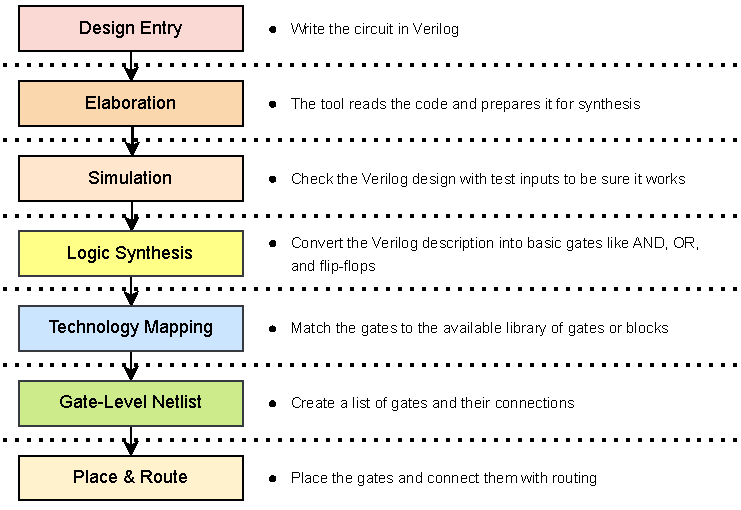
\includegraphics[width=\textwidth]{verilog_synthesis}
  \end{column}
  \end{columns}
\end{frame}

%===============================================================================
\section{Reading Verilog}
%===============================================================================

\begin{frame}{Reading Verilog: The Basics}
  \begin{itemize}\small\itemsep3pt
    \item \alert{Modules}: every circuit is a \texttt{module ... endmodule}; \texttt{input} and \texttt{output} declarations are the pins.
    \item \alert{Vectors}: \texttt{[7:0]} is a bus of 8 wires numbered 7 down to 0.
    \item \alert{assign}: a continuous, always-active connection: \texttt{assign y = a \& b;}
    \item \alert{Gate primitives}: \texttt{and}, \texttt{or}, \texttt{not}, \texttt{buf} instantiate gates like a schematic.
  \end{itemize}
  \centering\small\striped
  \begin{tabular}{@{}cl@{}}
    \toprule
    \texttt{3'b101} & 3-bit binary, decimal 5 \\ \texttt{8'hFF} & 8-bit hex, decimal 255 \\ \texttt{4'd9} & 4-bit decimal 9 \\
    \bottomrule
  \end{tabular}
  \begin{itemize}\small
    \item Format: \texttt{<size>'<base><value>}.
  \end{itemize}
\end{frame}

\begin{frame}{Operators}
  \begin{columns}[t]
  \begin{column}{.33\textwidth}
    \centering\small\striped
    \begin{tabular}{@{}cl@{}}
      \toprule
      \multicolumn{2}{c}{\textbf{Bitwise (per bit)}} \\
      \midrule
      \texttt{\&} & AND \\ \texttt{|} & OR \\ \texttt{\string~} & NOT \\ \texttt{\string^} & XOR \\
      \bottomrule
    \end{tabular}
  \end{column}
  \begin{column}{.38\textwidth}
    \centering\small\striped
    \begin{tabular}{@{}cl@{}}
      \toprule
      \multicolumn{2}{c}{\textbf{Reduction (bus to 1 bit)}} \\
      \midrule
      \texttt{\&d} & 1 if all bits of \texttt{d} are 1 \\ \texttt{|d} & 1 if any bit is 1 \\ \texttt{\string^d} & 1 if an odd number of bits are 1 \\
      \bottomrule
    \end{tabular}
  \end{column}
  \begin{column}{.27\textwidth}
    \centering\small\striped
    \begin{tabular}{@{}cl@{}}
      \toprule
      \multicolumn{2}{c}{\textbf{Other}} \\
      \midrule
      \texttt{?:} & conditional: 2-to-1 mux \\
      \bottomrule
    \end{tabular}
  \end{column}
  \end{columns}
  \vspace{2mm}
  \small\texttt{y = cond ? a : b;} means: if \texttt{cond} is 1, \texttt{y = a}; otherwise \texttt{y = b}.
\end{frame}

%===============================================================================
\section{Combinational Circuits}
%===============================================================================

\begin{frame}{Modeling Styles}
  \begin{itemize}\small\itemsep4pt
    \item \alert{Structural}: instantiate and connect components (gate primitives or modules); mirrors hierarchical hardware.
    \item \alert{Gate-level}: structural with primitive gates only; closest to a schematic. Best for learning.
    \item \alert{Dataflow}: Boolean expressions with \texttt{assign}; concise, focuses on function.
    \item \alert{Behavioral}: \texttt{always} blocks with \texttt{if} and \texttt{case}; the highest level, best for complex or sequential logic.
  \end{itemize}
  \begin{block}{Learning path}
    \small Start gate-level to build intuition, move to dataflow for compact code, use structural for larger systems, and behavioral for complex or sequential functions.
  \end{block}
\end{frame}

\begin{frame}[fragile]{2-to-1 Multiplexer}
  \begin{columns}[t]
  \begin{column}{.5\textwidth}
\begin{lstlisting}
module mux2to1_gate (
  input a, b, sel,
  output y
);
  wire nsel, w1, w2;
  not (nsel, sel);
  and (w1, a, nsel);
  and (w2, b, sel);
  or  (y, w1, w2);
endmodule
\end{lstlisting}
    \centering\vspace{1mm}
    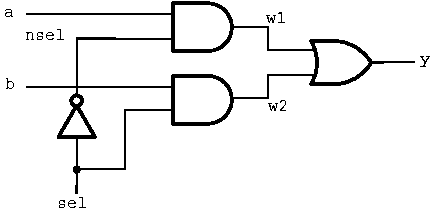
\includegraphics[height=.22\textheight]{verilog_mux2to1}
  \end{column}
  \begin{column}{.48\textwidth}
    \small Gate-level: \texttt{not} makes the inverted select, two \texttt{and} gates enable the chosen input, \texttt{or} combines them.
\begin{lstlisting}
module mux2to1_df (
  input a, b, sel,
  output y
);
  assign y = (sel) ? b : a;
endmodule
\end{lstlisting}
    \small Dataflow: one conditional operator.
  \end{column}
  \end{columns}
\end{frame}

\begin{frame}[fragile]{4-to-1 Multiplexer}
  \begin{columns}[t]
  \begin{column}{.52\textwidth}
\begin{lstlisting}
module mux4to1_gate (
  input a, b, c, d,
  input [1:0] sel,
  output y
);
  wire n0, n1, w1, w2, w3, w4;
  not (n0, sel[0]);
  not (n1, sel[1]);
  and (w1, a, n1, n0);
  and (w2, b, n1, sel[0]);
  and (w3, c, sel[1], n0);
  and (w4, d, sel[1], sel[0]);
  or  (y, w1, w2, w3, w4);
endmodule
\end{lstlisting}
  \end{column}
  \begin{column}{.46\textwidth}
\begin{lstlisting}
module mux4to1_df (
  input a, b, c, d,
  input [1:0] sel,
  output y
);
  assign y = (sel == 2'b00) ? a :
             (sel == 2'b01) ? b :
             (sel == 2'b10) ? c : d;
endmodule
\end{lstlisting}
    \small Gate-level: inverted selects, four \texttt{and} gates, one \texttt{or}. Dataflow: nested conditional operators.
  \end{column}
  \end{columns}
\end{frame}

\begin{frame}[fragile]{2-to-4 Decoder}
  \begin{columns}[t]
  \begin{column}{.52\textwidth}
\begin{lstlisting}
module dec2to4_gate (
  input [1:0] a,
  output [3:0] y
);
  wire na0, na1;
  not (na0, a[0]);
  not (na1, a[1]);
  and (y[0], na1, na0);   // 00
  and (y[1], na1, a[0]);  // 01
  and (y[2], a[1], na0);  // 10
  and (y[3], a[1], a[0]); // 11
endmodule
\end{lstlisting}
  \end{column}
  \begin{column}{.46\textwidth}
\begin{lstlisting}
module dec2to4_df (
  input [1:0] a,
  output [3:0] y
);
  assign y = 4'b0001 << a;
endmodule
\end{lstlisting}
    \small Gate-level: inverted inputs and four \texttt{and} gates give one-hot outputs. Dataflow: shift a one-hot value left by the input index.
  \end{column}
  \end{columns}
\end{frame}

\begin{frame}[fragile]{Half Adder and Full Adder}
  \begin{columns}[t]
  \begin{column}{.5\textwidth}
\begin{lstlisting}
module half_adder (
  input a, b,
  output sum, carry
);
  xor (sum, a, b);
  and (carry, a, b);
endmodule
\end{lstlisting}
\begin{lstlisting}
module half_adder_df (
  input a, b,
  output sum, carry
);
  assign sum   = a ^ b;
  assign carry = a & b;
endmodule
\end{lstlisting}
  \end{column}
  \begin{column}{.48\textwidth}
\begin{lstlisting}
module full_adder_gate (
  input a, b, cin,
  output sum, cout
);
  wire s1, c1, c2;
  half_adder ha1 (a, b, s1, c1);
  half_adder ha2 (s1, cin, sum, c2);
  or (cout, c1, c2);
endmodule
\end{lstlisting}
\begin{lstlisting}
module full_adder_df (
  input a, b, cin,
  output sum, cout
);
  assign {cout, sum} = a + b + cin;
endmodule
\end{lstlisting}
  \end{column}
  \end{columns}
\end{frame}

\begin{frame}{Structural Full Adder}
  \begin{columns}[c]
  \begin{column}{.55\textwidth}
    \centering
    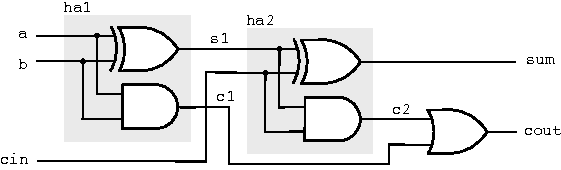
\includegraphics[width=\textwidth]{verilog_full_adder_gate}
  \end{column}
  \begin{column}{.43\textwidth}
    \begin{itemize}\small\itemsep3pt
      \item Built from \alert{two half-adder modules} and an OR gate.
      \item \texttt{ha1} adds \texttt{a} and \texttt{b}; \texttt{ha2} adds that sum and \texttt{cin}; the OR combines the two carries.
      \item Internal wires \texttt{s1}, \texttt{c1}, \texttt{c2} carry the intermediate signals.
      \item The dataflow version uses concatenation: \texttt{\{cout, sum\} = a + b + cin}.
    \end{itemize}
  \end{column}
  \end{columns}
\end{frame}

\begin{frame}[fragile]{2-Bit Comparator}
  \begin{columns}[t]
  \begin{column}{.56\textwidth}
\begin{lstlisting}
module comp2bit_gate (
  input [1:0] a, b,
  output eq, gt, lt
);
  wire eq1, eq0, gt1, gt0, lt1, lt0;
  xnor (eq1, a[1], b[1]);
  xnor (eq0, a[0], b[0]);
  and (eq, eq1, eq0);
  and (gt1, a[1], ~b[1]);
  and (gt0, eq1, a[0], ~b[0]);
  or  (gt, gt1, gt0);
  and (lt1, ~a[1], b[1]);
  and (lt0, eq1, ~a[0], b[0]);
  or  (lt, lt1, lt0);
endmodule
\end{lstlisting}
  \end{column}
  \begin{column}{.42\textwidth}
\begin{lstlisting}
module comp2bit_df (
  input [1:0] a, b,
  output eq, gt, lt
);
  assign eq = (a == b);
  assign gt = (a > b);
  assign lt = (a < b);
endmodule
\end{lstlisting}
    \small Gate-level: \texttt{eq} when both bits match; \texttt{gt} when the first mismatched bit of \texttt{a} is larger; \texttt{lt} likewise for \texttt{b}. Dataflow: comparison operators state the intent directly.
  \end{column}
  \end{columns}
\end{frame}

\begin{frame}[fragile]{8-to-3 Priority Encoder}
  \begin{columns}[t]
  \begin{column}{.46\textwidth}
    \small Gate-level: OR gates form the code directly.
\begin{lstlisting}
module prienc8to3_gate (
  input  [7:0] d,
  output [2:0] y,
  output valid
);
  or (valid, d[0], d[1], d[2], d[3],
             d[4], d[5], d[6], d[7]);
  or (y[2], d[7], d[6], d[5], d[4]);
  or (y[1], d[7], d[6], d[3], d[2]);
  or (y[0], d[7], d[5], d[3], d[1]);
endmodule
\end{lstlisting}
  \end{column}
  \begin{column}{.52\textwidth}
    \small Behavioral: priority is the order of the \texttt{if} conditions.
\begin{lstlisting}
module prienc8to3_beh (
  input  [7:0] d,
  output reg [2:0] y,
  output valid
);
  always @(*) begin
    if      (d[7]) y = 3'b111;
    else if (d[6]) y = 3'b110;
    else if (d[5]) y = 3'b101;
    else if (d[4]) y = 3'b100;
    else if (d[3]) y = 3'b011;
    else if (d[2]) y = 3'b010;
    else if (d[1]) y = 3'b001;
    else           y = 3'b000;
  end
  assign valid = |d;
endmodule
\end{lstlisting}
  \end{column}
  \end{columns}
  \vspace{1mm}
  {\small To change which input has priority, reorder the conditions instead of re-deriving the Boolean equations.}
\end{frame}

\begin{frame}[fragile]{Hazards and Buffers}
  \begin{columns}[t]
  \begin{column}{.5\textwidth}
    \small $Y = A\cdot B + \overline{A}\cdot C$ is functionally correct, but unequal gate delays can glitch $Y$ when $A$ changes (a \alert{static-1 hazard}). The reliable fix is the \alert{consensus term}: $Y = AB + \overline{A}C + BC$ holds $Y$ high while the two terms swap roles.
\begin{lstlisting}
module hazard_demo (
  input A, B, C,
  output Y
);
  wire nA, w1, w2;
  not (nA, A);
  and (w1, A, B);
  and (w2, nA, C);
  or  (Y, w1, w2);
endmodule
\end{lstlisting}
    \centering
    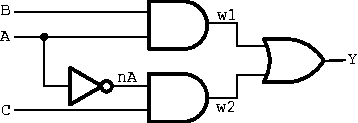
\includegraphics[height=.1\textheight]{verilog_hazard_prone}\hspace{2mm}
    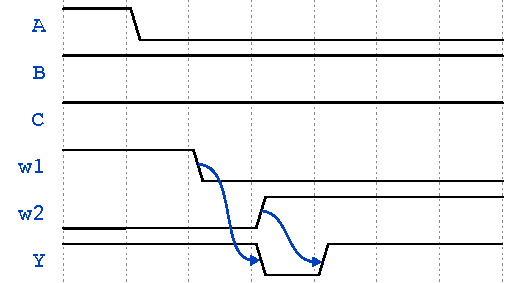
\includegraphics[height=.17\textheight]{verilog_hazard_prone_timing}
  \end{column}
  \begin{column}{.48\textwidth}
    \small A weaker approach: a \texttt{buf} delays $A$ in the first product term, balancing arrival times with $\overline{A}$:
\begin{lstlisting}
module hazard_free_demo (
  input A, B, C,
  output Y
);
  wire nA, Abuf, w1, w2;
  not (nA, A);
  buf (Abuf, A);
  and (w1, Abuf, B);
  and (w2, nA, C);
  or  (Y, w1, w2);
endmodule
\end{lstlisting}
    \centering
    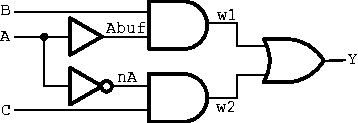
\includegraphics[height=.1\textheight]{verilog_hazard_free}\hspace{2mm}
    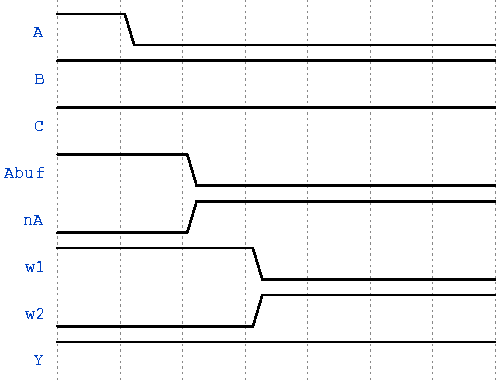
\includegraphics[height=.17\textheight]{verilog_hazard_free_timing}
  \end{column}
  \end{columns}
  \vspace{1mm}
  {\footnotesize Delay balancing reduces the likelihood of a glitch. It is an illustration, not a dependable fix: the delay depends on the technology, and synthesis may remove the buffer.}
\end{frame}

%===============================================================================
\section{Sequential Circuits}
%===============================================================================

\begin{frame}{Sequential Verilog}
  \begin{itemize}\small\itemsep4pt
    \item \alert{Question to keep in mind}: which values are stored, and what event makes them update?
    \item Sequential logic stores state in flip-flops or latches. It is written in \alert{behavioral} Verilog: \texttt{always @(posedge clk)} (or \texttt{negedge}) describes clocked updates; \texttt{if} and \texttt{case} give reset, enable and transitions.
    \item Naming: lowercase (\texttt{d}, \texttt{q}, \texttt{clk}) for single bits; uppercase or wider (\texttt{Q}, \texttt{DATA[7:0]}) for buses.
  \end{itemize}
  \begin{alertblock}{Simulation $\ne$ arbitrary software}
    \small Delays (\texttt{\#}), dynamic arrays, floating-point literals and \texttt{\$display} are accepted by simulators but cannot be synthesised. The synthesis report decides.
  \end{alertblock}
\end{frame}

\begin{frame}[fragile]{SR Latch and D Latch}
  \begin{columns}[t]
  \begin{column}{.48\textwidth}
    \small Level-sensitive, responds immediately to \texttt{S} and \texttt{R}:
\begin{lstlisting}
module sr_latch (
  input S, R,
  output reg Q
);
  always @(*) begin
    if (S && !R) Q = 1;      // Set
    else if (!S && R) Q = 0; // Reset
    // S=R=0: hold; S=R=1: invalid
  end
endmodule
\end{lstlisting}
  \end{column}
  \begin{column}{.5\textwidth}
    \small Transparent when \texttt{en} is high, otherwise holds:
\begin{lstlisting}
module d_latch (
  input D, en, reset,
  output reg Q
);
  always @(*) begin
    if (reset)   Q = 0;
    else if (en) Q = D; // transparent
    // else hold value
  end
endmodule
\end{lstlisting}
  \end{column}
  \end{columns}
\end{frame}

\begin{frame}[fragile]{D, T and JK Flip-Flops}
  \begin{columns}[t]
  \begin{column}{.32\textwidth}
    \small D: samples \texttt{D} on the rising edge.
\begin{lstlisting}
module d_ff (
  input D, clk, reset,
  output reg Q
);
  always @(posedge clk
           or posedge reset)
    if (reset) Q <= 0;
    else       Q <= D;
endmodule
\end{lstlisting}
  \end{column}
  \begin{column}{.32\textwidth}
    \small T: toggles when \texttt{T = 1}.
\begin{lstlisting}
module t_ff (
  input T, clk, reset,
  output reg Q
);
  always @(posedge clk
           or posedge reset)
    if (reset)  Q <= 0;
    else if (T) Q <= ~Q;
endmodule
\end{lstlisting}
  \end{column}
  \begin{column}{.34\textwidth}
    \small JK: set, reset, toggle.
\begin{lstlisting}
module jk_ff (
  input J, K, clk, reset,
  output reg Q
);
  always @(posedge clk
           or posedge reset)
    if (reset) Q <= 0;
    else if (J && !K) Q <= 1;
    else if (!J && K) Q <= 0;
    else if (J && K)  Q <= ~Q;
endmodule
\end{lstlisting}
  \end{column}
  \end{columns}
  \vspace{2mm}
  {\small Asynchronous reset: \texttt{posedge reset} is in the sensitivity list. Use non-blocking assignment (\texttt{<=}) for every register update.}
\end{frame}

\begin{frame}[fragile]{4-Bit Counter and Shift Register}
  \begin{columns}[t]
  \begin{column}{.48\textwidth}
    \small Up-counter with asynchronous reset:
\begin{lstlisting}
module counter4 (
  input clk, reset,
  output reg [3:0] Q
);
  always @(posedge clk
           or posedge reset)
    if (reset) Q <= 4'b0000;
    else       Q <= Q + 1;
endmodule
\end{lstlisting}
  \end{column}
  \begin{column}{.5\textwidth}
    \small Shifts right, inserting \texttt{D} at the left:
\begin{lstlisting}
module shiftreg4 (
  input clk, reset, D,
  output reg [3:0] Q
);
  always @(posedge clk
           or posedge reset)
    if (reset) Q <= 4'b0000;
    else       Q <= {D, Q[3:1]};
endmodule
\end{lstlisting}
  \end{column}
  \end{columns}
\end{frame}

%===============================================================================
\section{Finite State Machines}
%===============================================================================

\begin{frame}{Level-to-Pulse Converter in Verilog}
  \begin{itemize}\small\itemsep3pt
    \item The Moore level-to-pulse FSM of Chapter 13: one single-cycle pulse per rising edge of \texttt{L}, however long \texttt{L} stays high.
    \item Three states:
    \begin{itemize}\small
      \item \texttt{ZERO}: waiting for \texttt{L} to rise; \texttt{P = 0}.
      \item \texttt{EDGE}: one cycle after the rising edge; \texttt{P = 1}.
      \item \texttt{ONE}: waiting for \texttt{L} to fall; \texttt{P = 0}.
    \end{itemize}
    \item From \texttt{EDGE}: to \texttt{ZERO} if \texttt{L = 0}, else to \texttt{ONE}: exactly one pulse per rising edge.
  \end{itemize}
  \begin{block}{Three-process structure}
    \small \alert{State register} (clocked), \alert{next-state logic} (combinational, a \texttt{case}), \alert{output logic} (combinational). Separating them gives a clear, synthesizable, maintainable design.
  \end{block}
\end{frame}

\begin{frame}[fragile]{The Three-Process FSM}
\begin{lstlisting}[basicstyle=\ttfamily\scriptsize]
module edge_detector (
  input  clk, reset,
  input  L,        // input level signal
  output P         // pulse output
);
  localparam [1:0] ZERO = 2'b00, EDGE = 2'b01, ONE = 2'b10;
  reg [1:0] state, next_state;

  // PART 1: State register
  always @(posedge clk or posedge reset)
    if (reset) state <= ZERO;
    else       state <= next_state;

  // PART 2: Next-state logic
  always @(*) begin
    case (state)
      ZERO: next_state = L ? EDGE : ZERO;
      EDGE: next_state = L ? ONE  : ZERO;
      ONE:  next_state = L ? ONE  : ZERO;
      default: next_state = ZERO;
    endcase
  end

  // PART 3: Output logic (Moore: depends only on state)
  assign P = (state == EDGE);
endmodule
\end{lstlisting}
  \small \texttt{default} gives a recovery path: two bits can encode four values but only three are used.
\end{frame}

\begin{frame}{Back to the Opening Question}
  \begin{block}{Why does ``C-like'' Verilog compile to gates?}
    \small Because Verilog describes \alert{structure and behaviour that exist concurrently}, not a sequence of instructions. \texttt{assign} makes combinational logic, \texttt{always @(*)} makes combinational logic from \texttt{if} or \texttt{case}, and \texttt{always @(posedge clk)} makes flip-flops. The synthesis tool turns those descriptions into gates and registers; there is no CPU to execute them.
  \end{block}
  \begin{block}{Which values are stored, and what updates them?}
    \small What is stored is whatever is assigned in the \texttt{always} block and declared \texttt{reg}; the event is named in the sensitivity list. \texttt{always @(posedge clk)}: a rising edge, so a flip-flop. \texttt{always @(*)}: no event; it re-evaluates when any input changes. The latch examples infer latches deliberately, despite the warning in the Summary.
  \end{block}
\end{frame}

%===============================================================================
\section{Summary}
%===============================================================================

\begin{frame}{Summary}
  \begin{itemize}\itemsep3pt\small
    \item A Verilog file describes \alert{hardware that exists concurrently}, not a program run top to bottom.
    \item Combinational: \texttt{assign} for simple expressions; \texttt{always @(*)} for \texttt{case}/\texttt{if} logic. Every path must assign every output, or synthesis infers unintended latches.
    \item Sequential: \texttt{always @(posedge clk)} with non-blocking assignment (\texttt{<=}) for every register update; keep reset style consistent.
    \item FSMs are cleanest as three processes: state register, next-state logic, output logic. Add a \texttt{default} to every \texttt{case}.
    \item Simulation checks behaviour; synthesis checks implementability. A passing simulation does not guarantee a working chip.
  \end{itemize}
  \begin{block}{Looking ahead}
    This is a first step. A full HDL course covers parameterised modules, timing closure, clock-domain crossings and SystemVerilog. Next: take a small design from Chapters 9--15, write it in Verilog, simulate it and synthesise it onto an inexpensive FPGA board.
  \end{block}
\end{frame}

\end{document}
